\documentclass
[
	12pt,
	a4paper,
	oneside,
%	titlepage
]{article}
%titlepage prints the title on it's own page in article class

%doublespace my text
\renewcommand{\baselinestretch}{1.5}

%reduce the hyphenation of words
\sloppy

%prints a small space between paragraphs and removes the indenting of the first line
\setlength{\parskip}{2ex plus0.5ex minus 0.2ex}
\setlength{\parindent}{0em}

%csquotes - provides multilingual quoting - keeps babel happy
\usepackage{csquotes}
%babel required for biblatex to work. Specifying british last make it the language in use
%\usepackage[english,british]{babel}
\usepackage[british]{babel}

\usepackage[style=authoryear,backend=biber,
	giveninits=true,
	uniquename=init,
	citestyle=authoryear,
	language=british]{biblatex}

%Add a comma between name and year in citations
\renewcommand*{\nameyeardelim}{\addcomma\space}

\usepackage{graphicx}

\usepackage{amsthm}
\newtheorem*{nullhypothesis}{Null hypothesis}

\defbibnote{needsfixing}{\emph{(this formatting needs looking at -- not currently to LSBU standards.
For example, need to include names of all the authors.)}}
% Add my bibliography file here
\addbibresource{references.bib}

%rotating allows text to be printed sideways
%multirow allows tables with cells spanning more than one row
% Remove this if not required
%\usepackage{rotating,multirow}


\begin{document}
\author{Gregory Cartwright}
\title{Does level of frailty influence preemtive planning of treatment escalation 
	for community hospital inpatients?
}
\maketitle
\begin{abstract}
\emph{The abstract goes here.}
\end{abstract}
\section{Introduction}

%\subsection{Context}
The population of the UK is getting older and this is trend is forecast to continue.
In 2016 18\% of the population was over 65 years old, with 2.4\% over 85 years old.
Both these figures are expected to grow over the next 20 years \parencite{ons:17}.
Frailty is widely agreed to be a condition where the maintenance of homeostasis 
becomes vulnerable to 
small stressors \parencite{vellas:16}.  Examples of such stressors include changes in environment and minor
illness. The consequences of exposure to these include delirium, significant reduction in mobility,
falls, increased dependency, non-specifc failure to thrive and death 
\parencite{bgs:14,vellas:16,oliver:14}.
The prevalence of frailty amongst the ageing population is high \parencite{clegg:13},
with about 10\% of those aged over 65 and up to 50\% of
those aged over 85\% having frailty \parencite{bgs:14}. These figures
are thought to be higher still in the group of people that are housebound, 
have care at home or live in a care home \parencite{oliver:14}.

The author is an advanced nurse practitioner (ANP) in a community Trust.
The Trust has community hospitals which have wards for inpatient rehabilitation and
medical stepdown. There are 12 wards accross 8 community hospitals. Each ward has
an ANP who works on the ward to provide medical management of the patients during 
the hours of Monday to Friday, 0900 to 1730. Outside of these hours, medical care 
is provided by the out of hours (OOH) general practitioner (GP) service. 

Most patients are admitted to the community hospital wards for either rehabilitation
or medical stepdown. The majority of these patients come following an acute admission
where they have been stabilised medically but are often deconditioned as a result
of acute illness and are not ready to go home. At this stage their needs include 
ongoing medcial treatment and monitoring and further assessments and treament such 
as physiotherapy and occupational therapy to prepare them for discharge home.

Some patients are admitted directly from home because they have medical or rehabilitation
needs that cannot be met at home but do not require an admission to an acute setting.
A minority of patients are admitted for paliative care.

When patients are admitted to one of these wards they have a comprehensive geriatric 
assessment (CGA) \parencite{bgs:14} performed by the multi-disciplinary team (MDT).
An international meta-analysis found that, when compared with general medical care,
CGA was effective at keeping older people alive and living in their own homes at
twelve months post admission with a number needed to treat of 33 \parencite{ellis:11}.

The author expects that many of the patients admitted to the wards have frailty.
The numbers of patients with frailty is not known, however the patients are assessed 
for frailty and the patients admitted are old. During the last financial year the
average age was 81 and 49\% of patients admitted were aged 85 or over. Many have 
care needs as seen above.

Although the patients are usually clinically stable when they arrive on the ward,
their condition can deteriorate. This is usually managed in the community hospital
ward environment, where treaments such as intravenous (IV) fluids, IV antibiotics
and even blood transfusions can be given. Sometimes the deterioration is such that, 
for optimal management, services are required that can only be offered in secondary 
care. When this is the case the patient is transferred to an acute hospital as an
urgent or emergency case. The decision as to whether this course of action is required
is taking by the ANP who may liaise with the the consultant geriatrician. During
the OOH period this decision is made by the OOH GP.

There is evidence that patients with frailty often have poor outcomes, including death,
following admission to acute hospital \parencite{silver:12, wallis:15}. The ANPs
are aware of this, and when they recognise that someone is particularly frail, they
will have discussions with the patient and their family about the relative risks
and benefits of a potential admission to an acute hospital and what they would want to 
happen in the event of deterioration in their health. This way plan can be made 
before any deterioration happens.

When patients deteriorate during the OOH period and the patient
gets sent to the acute Trust, the ANP reviews what happened to see if the admission
could have been avoided. There are times when the ANP feels that, in those particular
circumstances, the risks to the patient of the acute admission outweigh the benefits
due to their frailty, and that the patient should have preemtive planning of 
escalation of care earlier in their stay to avoid this acute admission.

The level of frailty of patients is recorded but not used to guide planning of
treament escalation. This project aims to examine if frailty guides preemetive
planning of treatment escalation in these community hospitasl inpatients.

\section{Literature review}

\emph{(Need to write about literature search strategy that was employed.)}

\subsection{Assessing frailty}
An international systematic review found 
that at least 10\% of people aged over 65 had frailty and of those aged 85 or over
at least 26\% were frail \parencite{collard:12}. There are various methods and tools used to assess frailty.
Some of these count the number of deficits from a particular set that a person has. 
\textcite{sternberg:08} suggest that such a tool is not practical for use in a clinical
setting, being more suitable to assessing populations for strategic planning. 
Other tools require numerous specific measurements to be taken, again making them
less suitable for clinical use \parencite{martin:08} and possibly more suited to research purposes
\parencite{ensrud:08}. \textcite{romero-ortuno:16} argue that this fragmentation should not
be viewed as a problem as each frailty assessment tool is suited to a different 
purpose. 

In both the clincal area which the author works and the emergency department at
the local acute Trust, frailty is assessed using the Clinical Frailty Scale (CFS).
See appendix~\ref{appendix:CFS}.
The CFS is a tool that has been validated for use in cinical practice 
\parencite{rockwood:05}. It rates frailty based on the person's level of independence
and dependence, giving them an ordinal postion on the continuum from very fit and completely 
independent, CFS of 1, to very severely frail and completely dependent, CFS of 8.
There is also a CFS of 9 for those who are terminally ill. The CFS is based on clinical
judgment of the patient and is therefore suited to clinical use, certainly after
the patient has had a CGA \parencite{bgs:14}.

Generally, the majority of the population of community hospitals is frail older 
people \parencite{silver:12}.
The CFS score has recently been introduced to the community hospital wards in the author's Trust. The
score is not being used for any specific purpose, it is just being entered into 
the patients' notes for people to refer to. These scores are not being collected, 
but the author suspects that the proportion of inpatients who are at least 
moderately frail, with CFS at least 6, will be quite high. Specifically because
CFS is partly based on a person's ability to carry out activities of daily living (ADLs)
and instumental activities of daily living (IADLs) and one reason that many patients
are admitted to the community hospital is that they need rehabilitation to be
able to carry out ADLs and IADLs. Indeed in a study to assess the prevalence of frailty
in France, \textcite{cossec:16} found that dependency on others for IADLs was an 
independent determinant of frailty.

\subsection{Consequences of frailty}

By definition, frailty is a state where a small change, intrinsic or extrinsic, can
lead to multiple consequences \parencite{collard:12}. These can be severe, including 
death. An examination
of all bereavements of adults in England that were not due to accident, homicide or suicide for 
a four month period in 2012 was 
carried out \parencite{ons:13}. It found that the proportion of deaths
that were not due to cancer or any cardiovascular disease was 42\%. In the over 80
age group this was 80\%. The most recent edition of this survey from 2015 found
that the overall proportion of non-cancer and non-CVD deaths was slightly higher 
at 46\% \parencite{ons:16}, but did not provide a breakdown by age group. They 
did however report that 60\% of their sample were aged over 80.

How many of these deaths were due to frailty is not know, however 
a Canadian study that examined all deaths in Alberta found that frailty was the
cause of 30\% of mortality \parencite{fassbender:09}.

A national guide for emergency and urgent care of older people \parencite{silver:12}
reports that many older people are admitted to hospital only to die within hours.
This is particularly true during for people admitted during the out of hours period.
Whilst this does not quantify the sequelae of frailty, there is literature that 
supports this. \textcite{wallis:15} performed a retrospective study looking 
at outcomes of hosptial admission for people aged 75 and over, in relation to CFS. 
They found that increased frailty was an independent predictor of both 30-day
readmission and in-patient death, with nearly a quarter of people with CFS of 8 dying 
during the admission. This supports the work of \textcite{kang:15} whose Chinese 
study also found that frailty was independtly associated with an increased risk of 
inpatient death, and also significantly increased the risk of readmission and 
3-month mortality for those who survived to hospital discharge.

The effect of frailty on those discharged from hospital was also studied by 
\parencite{kahlon:15}, who also found that frailty significantly increased the 
risk of both readmission and death within 30 days of discharge.

\subsection{Interventions for frailty}
Frailty is clearly a problem, so what should be done about it? Older patients 
should be screened for frailty at every contact with a health professional 
\parencite{bgs:14}, and 
this is already happening in the community hospital wards. There is a consensus that 
frailty should be viewed as a syndrome with multiple domains and therefore
there should be an MDT approach to it's management \parencite{vellas:16}.

The CGA is a multidisciplinary, evidence based strategy to guide the management 
of frailty that is viewed as best practice \parencite{silver:12, bgs:14, oliver:14}. Patients
in the communtity hospitals already recieve this regardless of their CFS score.

We have seen how frailty combined with illness carries a high risk of death, and 
\textcite{silver:12} report that end of life care in older people with frailty
is something that is often not adequately considered. \textcite{oliver:14} support this
by asserting that people with frailty are often not involved in planning their 
end-of-life care. They suggest that the reasons for this include factors such as
the trajectory, with frailty often being a more gradual decline without sudden 
landmark moments. This contrasts with conditions such as terminal cancer where there 
is a defining transition to an end-of-life phase. This can mean that entering such a
phase is not recognised and therefore planning is overlooked. 

Should the recognition of a high level of frail act as an event to signify
that a person is entering an end-of-life phase? Having found that frailty in the 
context of acute coronary syndrome is associated
with poor outcomes, \textcite{kang:15} recommend that a high CFS should
trigger the consideration planning of escalation pathways \parencite{kang:15}.
This supports the recommendations of \textcite{silver:12} who assert that over-investigation
and uncessary interventions in the frail elderly population are costly to both the
individual and the health economy. They go on to advise that in such patients, 
their preferences for their future care should be ascertained early. \textcite{oliver:14} 
reinforce this by highlighting the importance of gathering this information
before the person loses the capacity to make decisions about how their care should
progress. The later work of \textcite{romero-ortuno:16} add weight to this argument.
Having identified the increased risk associated with frailty and hospital admission, 
they recommend that frailty generally should trigger personalised planning of
care and it's escalation.

\section{Aim and objectives}
\subsection{Framing the problem}
As mentioned previously, outside the hours of 9am to 5pm monday to friday, the medical
care of patients in the community hospital wards where the author works is provided
by the local OOH GP service. When a patient
is referred to this service, the GP normally has no prior knowledge of the patient. They are
given a telephone handover by the referring nurse and using that information
they have to triage the patient. A decision has to be made as to whether they should visit
the patient to review them clinically, or if they are too unwell for this and they 
should be taken to an emergency department (ED). These patients
are already in a hospital environment where many acute conditions can be managed.
Basic investigations such as blood tests and in-hours xrays can be obtained from the community
ward and treaments including IV antibiotics and IV fluids can be given.
To make a decision about escalation of care environment for a deteriorating patient
requires a risk benefit analysis to be carried out. 

During the OOH period this is 
made more difficult because the patient is not known to the practitioner, the patient
is acutely unwell so may not be able to participate in discussions about their care,
relatives may not be easy to contact if it is nighttime. In these circumstances it could
be argued that the safest option is to admit the patient to the ED where their 
condition can be further assessed and closely monitored. 

We have seen above that outcomes for people with frailty who are admitted to hospital
are often poor. The \textcite{silver:12} assert that during the OOH period many older
people with frailty are admitted to hospital only to die shortly after, sometimes within
hours. The author feels that, in his work environment, there are often 
patients who get admitted to ED during the OOH period where the level or their frailty
means that the risks presented to them by an admission to an acute hospital are great
and sometimes outweight the benefits offered by such a transfer of care. This has
been noticed in retrospect. The frailty of these patients is assessed on admission
to the wards. Most of these patients come for rehabilitation or as a medical stepdown,
so are usually medically stable when they are admitted to the ward. Their frailty 
is assessed at this point, so if they are found to be severly frail, this would
seem like an ideal point in their journey to review their plan of care including
what they would like to happen and what would be the most appropriate course of 
action if their condition were to deteriorate.

This is done for some of the patients, but clearly not all who would benefit from it. 
Deciding whether to do this planning or not is not currently formally triggered 
by their level of frailty, however, the risks that we have seen above of acute hospital 
admission for people with frailty are great. This suggests that identifying severe frailty 
should trigger consideration of preemtive planning of treatment escalation.

\subsection{Aim}
This raises the question that if a person is admitted to a community hospital, has 
severe frailty and does not already have a treament escalation plan in place when they 
arrive on the ward, is the planning of treatment escalation considered? The overall 
aim of this study will be to examine if the level of frailty of community hospital
in-patients influences the consideration of preemtive planning of escalation of 
treatment.

\subsection{Objectives}

The objectives are as follows:
\begin{enumerate}
\item	Critically evaluate the likely outcomes for community hospital patients 
		with levels of frailty and acute illness. \label{obj:background}
\item	Ascertain the prevalence of levels of frailty within the local community
		hospital population. \label{obj:prevalence}
\item	Identify the proportion of patients with frailty that is at least moderate
		that do not have a pre-existing plan for treament escalation. \label{obj:noplan}
\item	Identify how many of these patients have consideration of preemetive planning
		of treament escalation during their in-patient stay. \label{obj:association}
\item	Formulate local recommendations for practice to help reduce unhelpful
		acute hospital admissions for people with frailty through more effective
		preemtive planning of treatment escalation.
\end{enumerate}

\section{Study design} \label{sec:design}
To assess objective~\ref{obj:background} a literature review will be used. 
The remaining objectives require collection of numbers
and proportions of patients that meet objective criteria. A quantitative design
will be appropriate to this approach \parencite{parahoo:14}.

The study aims to examine the association between the independent variable of 
the level of frailty and the dependent variable of the whether preemtive planning
was carried out. It therefore seems appropriate to use a correlational design. 
It will be a retrospective observational 
cross-sectional study: current in-patient casenotes will be reviewed. To achieve objectives \ref{obj:prevalence}
and \ref{obj:noplan} data will be obtained by reviewing the case-notes
of patients, examining the initial MDT assessments to ascertain CFS score and 
whether a treament escalation plan was in place prior to admission. For objective~
\ref{obj:association}, the entire case-notes of patients will be reviewed to ascertain
whether preemetive planning of treament escalation was considered during the stay.

\section{Sample}
Time for data collection is limited due to the timescale for the dissertation. 
Therfore the sampling method needs to capture as many patients as possible in a 
short time. To facilitate this a convenience sampling method will be used.

An electronic patient record (EPR) is currently being rolled out across the Trust.
Currently eight out of the twelve wards have this implemented, so all the patient 
records for patients on these wards are accessible by the author remotely. This
accounts for 148 of the total of 214 beds: 69\%. All patients on these wards with
EPR will be the sample.


\section{Research instruments and procedure}
Due to time constraints, data will be collected by taking a snapshot on each ward 
of the patients. Within the first week of their stay patients will have been reviewed
by all members of the MDT including the geriatrician, so the team should be aware 
of the patient's frailty and had chance to consider the approiateness of potential 
treatment escalation. The average length of stay (LOS) is 20.4 days, so very few 
will have been discharged within one week.

For each of these patients, the EPR will be reviewed as set out in 
section~\ref{sec:design}. For objectives \ref{obj:prevalence} and \ref{obj:noplan} 
the initial admission and clerking documentation will be reviewed to access and 
record the CFS score and to see whether the patient has a pre-existing plan 
for treamtment escalation. This will be recorded.

To collect data for objective \ref{obj:association}, all patients who do not have
a pre-existing plan will then have their EPR searched
for the duration of their admission. The record will be searched for the following
terms:

\begin{itemize}
\item acute
\item escalation
\item advanced care plan
\item deterioration
\item \emph{(need to add to this list)}
\end{itemize}

Where one of these terms is found, the record will be read in context to assess if 
escalation planning was being considered.

The number of patients who did not have a treatment escalation plan before admission
to the community hospital and for whom escalation planning was subsequently considered will then be 
collated for each level on the CFS.

\section{Data analysis}
\emph{I need some help with this section}

\section{Ethical considerations}
\emph {Need to talk about submitting my plan to the Trust research department for
	approval }
\clearpage
\printbibliography[prenote=needsfixing]

\clearpage
\begin{appendix}
\section{Clinical Frailty Scale}
\label{appendix:CFS}
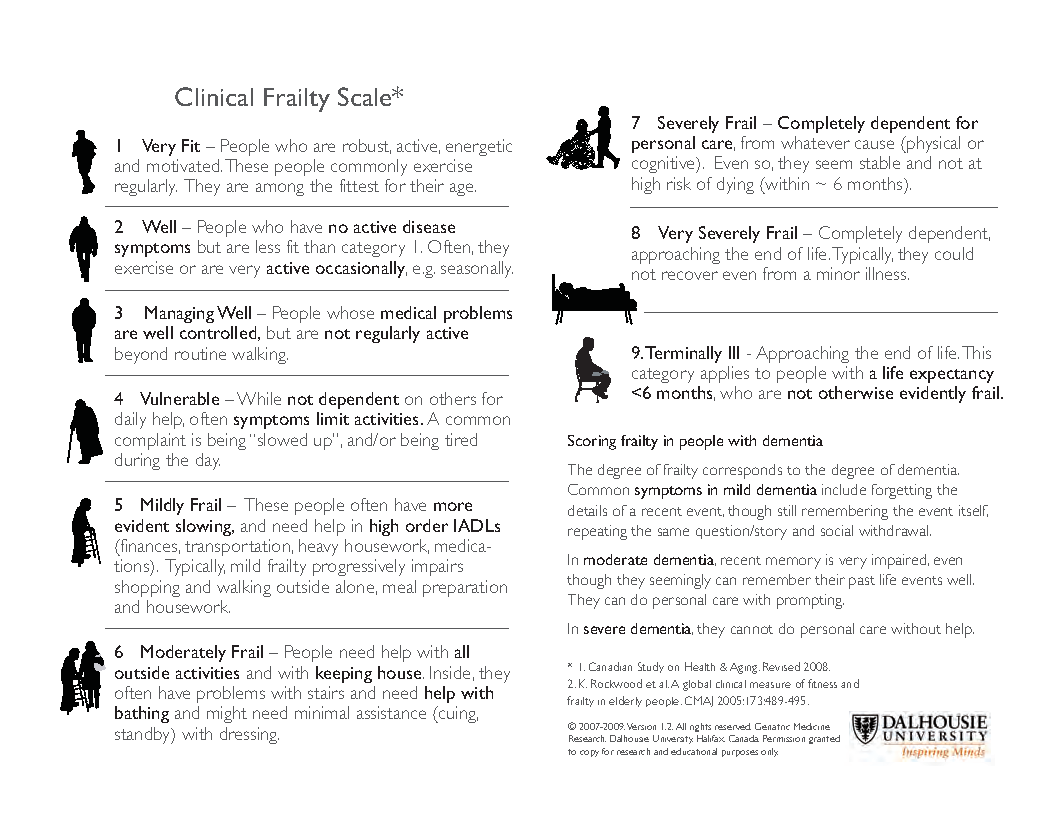
\includegraphics[width=\textwidth]{CFS}
\end{appendix}

\end{document}
